% !TeX program = lualatex
% このファイルは LuaLaTeX で処理してください(pdfLaTeX/upLaTeXでは動作しません)。
\documentclass[a4paper,11pt]{ltjsarticle}

\usepackage{amsmath,amssymb,mathtools}
\usepackage{siunitx}
\usepackage{geometry}
\geometry{a4paper,top=15mm,bottom=18mm,left=14mm,right=14mm}
\usepackage{tikz}
\usetikzlibrary{arrows.meta,positioning,calc}
\usepackage[most]{tcolorbox}
\usepackage{booktabs}
\usepackage{array}
\usepackage{enumitem}

\setlength{\parindent}{0pt}
\setlength{\parskip}{2pt}
\renewcommand{\arraystretch}{2.6}

\newcommand{\banner}[1]{%
  \begin{tcolorbox}[colback=black,coltext=white,boxrule=0pt,sharp corners,
    left=8pt,right=8pt,top=5pt,bottom=5pt,before skip=8pt,after skip=8pt]
    {\Large\bfseries #1}
  \end{tcolorbox}}

\newcommand{\subbanner}[1]{%
  \begin{tcolorbox}[colback=black!80,coltext=white,boxrule=0pt,sharp corners,
    left=8pt,right=8pt,top=4pt,bottom=4pt,before skip=6pt,after skip=6pt]
    {\large\bfseries #1}
  \end{tcolorbox}}

\newtcolorbox{pointbox}[1][]{%
  colback=black!4,colframe=black,boxrule=0.6pt,arc=1mm,
  left=6pt,right=6pt,top=4pt,bottom=4pt,#1}

\pagestyle{plain}

\begin{document}

\banner{気柱の振動 演習}

下の図は，長さ $\ell$ の管に生じる気柱の定常波のようすを表している(閉端の位置には黒い壁，節の位置には破線，開口端付近に見える点線は，節または腹の位置の目安として引いてある)。それぞれの図をよく見て，表の空欄をうめよ。音の速さを $V$ とする。

% ------------------------------------------------------
\subbanner{開管の振動}
\noindent\hspace{1.5cm}\begin{tabular}{c>{\centering\arraybackslash}p{2.4cm}|>{\centering\arraybackslash}p{2.2cm}|c}
\cline{2-4} % 表部分（2〜4列目）の上側の罫線。気柱の図の列には引かない

% ---- ヘッダー行 ----
\makebox[3.6cm][l]{\hspace{-1.2cm}\begin{tikzpicture}[x=1cm,y=1cm]
  \draw[<->,>=stealth] (0,0) -- (3.6,0); % 気柱（管）全体の長さ l を示す両矢印
  \node[font=\small] at (1.8,0.35) {$\ell\,[\mathrm{m}]$}; % 矢印の上に長さのラベルを表示
\end{tikzpicture}}
& % 振動の名称列（ヘッダー行なので空欄）
& \textbf{波長 $\lambda\,[\mathrm{m}]$} % 波長列の見出し
& \textbf{振動数 $f\,[\mathrm{Hz}]$} \\ % 振動数列の見出し
\cline{2-4} % ヘッダー行の下側の罫線（気柱の図の列には引かない）

% ---- 基本振動 (n=1) ----
\makebox[3.6cm][l]{\hspace{-1.2cm}\begin{tikzpicture}[x=0.6cm,y=0.6cm]
  \draw[thick] (0,1.3) -- (6,1.3); % 管の上側の壁を表す直線
  \draw[thick] (0,-1.3) -- (6,-1.3); % 管の下側の壁を表す直線
  \draw[dashed] (3,2.1) -- (3,-2.1); % 中央にある節の位置を示す点線
  \draw[dotted] (0,2.1) -- (0,-2.1); % 左端（開口端）にある腹の位置を示す点線
  \draw[dotted] (6,2.1) -- (6,-2.1); % 右端（開口端）にある腹の位置を示す点線
\end{tikzpicture}}
& & & \\
\cline{2-4} % この行の下側の罫線

% ---- 2倍振動 (n=2) ----
\makebox[3.6cm][l]{\hspace{-1.2cm}\begin{tikzpicture}[x=0.6cm,y=0.6cm]
  \draw[thick] (0,1.3) -- (6,1.3); % 管の上側の壁を表す直線
  \draw[thick] (0,-1.3) -- (6,-1.3); % 管の下側の壁を表す直線
  \draw[dashed] (1.5,2.1) -- (1.5,-2.1); % 1つ目の節の位置を示す点線
  \draw[dashed] (4.5,2.1) -- (4.5,-2.1); % 2つ目の節の位置を示す点線
  \draw[dotted] (0,2.1) -- (0,-2.1); % 左端（開口端）にある腹の位置を示す点線
  \draw[dotted] (3,2.1) -- (3,-2.1); % 中央（内部）にある腹の位置を示す点線
  \draw[dotted] (6,2.1) -- (6,-2.1); % 右端（開口端）にある腹の位置を示す点線
\end{tikzpicture}}
& & & \\
\cline{2-4}

% ---- 3倍振動 (n=3) ----
\makebox[3.6cm][l]{\hspace{-1.2cm}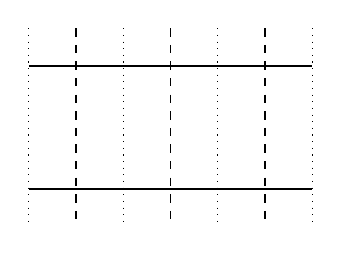
\begin{tikzpicture}[x=0.6cm,y=0.6cm]
  \draw[thick] (0,1.3) -- (6,1.3); % 管の上側の壁を表す直線
  \draw[thick] (0,-1.3) -- (6,-1.3); % 管の下側の壁を表す直線
  \draw[dashed] (1,2.1) -- (1,-2.1); % 1つ目の節の位置を示す点線
  \draw[dashed] (3,2.1) -- (3,-2.1); % 2つ目の節の位置を示す点線
  \draw[dashed] (5,2.1) -- (5,-2.1); % 3つ目の節の位置を示す点線
  \draw[dotted] (0,2.1) -- (0,-2.1); % 左端（開口端）にある腹の位置を示す点線
  \draw[dotted] (2,2.1) -- (2,-2.1); % 1つ目の内部の腹の位置を示す点線
  \draw[dotted] (4,2.1) -- (4,-2.1); % 2つ目の内部の腹の位置を示す点線
  \draw[dotted] (6,2.1) -- (6,-2.1); % 右端（開口端）にある腹の位置を示す点線
\end{tikzpicture}}
& & & \\
\cline{2-4}

% ---- 「以下同様に続く」ことを示す小さな区切り行 ----
\makebox[3.6cm][l]{\hspace{-1.2cm}\begin{tikzpicture}[x=0.6cm,y=0.6cm]
  \node[font=\small] at (3,0) {$\vdots$};
\end{tikzpicture}}
& $\vdots$ & $\vdots$ & $\vdots$ \\
\cline{2-4}

% ---- n倍振動（両端に2ループずつ表示、中央は「…」で省略） ----
\makebox[3.6cm][l]{\hspace{-1.2cm}\begin{tikzpicture}[x=0.6cm,y=0.6cm]
  \draw[thick] (0,1.3) -- (6,1.3); % 管の上側の壁を表す直線（全体）
  \draw[thick] (0,-1.3) -- (6,-1.3); % 管の下側の壁を表す直線（全体）
  \node[font=\small] at (3,0) {$\cdots$}; % 中央部分：多数のループが続くことを省略記号で示す
\end{tikzpicture}}
& & & \\
\cline{2-4}
\end{tabular}

\clearpage
% -------------------------------------------------------------------
\subbanner{閉管の振動}
\noindent\hspace{1.5cm}\begin{tabular}{c>{\centering\arraybackslash}p{2.4cm}|>{\centering\arraybackslash}p{2.2cm}|c}
\cline{2-4} % 表部分（2〜4列目）の上側の罫線。気柱の図の列には引かない

% ---- ヘッダー行 ----
\makebox[3.6cm][l]{\hspace{-1.2cm}\begin{tikzpicture}[x=1cm,y=1cm]
  \draw[<->,>=stealth] (0,0) -- (3.6,0); % 気柱（管）全体の長さ l を示す両矢印
  \node[font=\small] at (1.8,0.35) {$\ell\,[\mathrm{m}]$}; % 矢印の上に長さのラベルを表示
\end{tikzpicture}}
& % 振動の名称列（ヘッダー行なので空欄）
& \textbf{波長 $\lambda\,[\mathrm{m}]$} % 波長列の見出し
& \textbf{振動数 $f\,[\mathrm{Hz}]$} \\ % 振動数列の見出し
\cline{2-4}

% ---- 基本振動 (m=1) ----
\makebox[3.6cm][l]{\hspace{-1.2cm}\begin{tikzpicture}[x=0.6cm,y=0.6cm]
  \fill[black] (-0.08,-1.3) rectangle (0,1.3); % 閉端（固定壁）を表す黒い長方形
  \draw[thick] (0,1.3) -- (6,1.3); % 管の上側の壁を表す直線
  \draw[thick] (0,-1.3) -- (6,-1.3); % 管の下側の壁を表す直線
  \draw[dotted] (6,2.1) -- (6,-2.1); % 右端（開口端）にある腹の位置を示す点線
\end{tikzpicture}}
& & & \\
\cline{2-4}

% ---- 3倍振動 (m=3) ----
\makebox[3.6cm][l]{\hspace{-1.2cm}\begin{tikzpicture}[x=0.6cm,y=0.6cm]
  \fill[black] (-0.08,-1.3) rectangle (0,1.3); % 閉端（固定壁）を表す黒い長方形
  \draw[thick] (0,1.3) -- (6,1.3); % 管の上側の壁を表す直線
  \draw[thick] (0,-1.3) -- (6,-1.3); % 管の下側の壁を表す直線
  \draw[dashed] (4,2.1) -- (4,-2.1); % 管内部にある節の位置を示す点線
  \draw[dotted] (2,2.1) -- (2,-2.1); % 内部にある腹の位置を示す点線
  \draw[dotted] (6,2.1) -- (6,-2.1); % 右端（開口端）にある腹の位置を示す点線
\end{tikzpicture}}
& & & \\
\cline{2-4}

% ---- 5倍振動 (m=5) ----
\makebox[3.6cm][l]{\hspace{-1.2cm}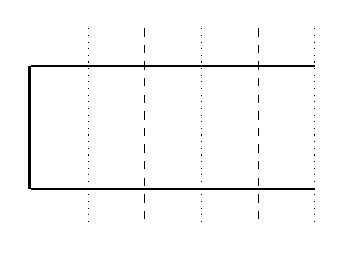
\begin{tikzpicture}[x=0.6cm,y=0.6cm]
  \fill[black] (-0.08,-1.3) rectangle (0,1.3); % 閉端（固定壁）を表す黒い長方形
  \draw[thick] (0,1.3) -- (6,1.3); % 管の上側の壁を表す直線
  \draw[thick] (0,-1.3) -- (6,-1.3); % 管の下側の壁を表す直線
  \draw[dashed] (2.4,2.1) -- (2.4,-2.1); % 1つ目の節の位置を示す点線
  \draw[dashed] (4.8,2.1) -- (4.8,-2.1); % 2つ目の節の位置を示す点線
  \draw[dotted] (1.2,2.1) -- (1.2,-2.1); % 1つ目の内部の腹の位置を示す点線
  \draw[dotted] (3.6,2.1) -- (3.6,-2.1); % 2つ目の内部の腹の位置を示す点線
  \draw[dotted] (6,2.1) -- (6,-2.1); % 右端（開口端）にある腹の位置を示す点線
\end{tikzpicture}}
& & & \\
\cline{2-4}

% ---- 「以下同様に続く」ことを示す小さな区切り行 ----
\makebox[3.6cm][l]{\hspace{-1.2cm}\begin{tikzpicture}[x=0.6cm,y=0.6cm]
  \node[font=\small] at (3,0) {$\vdots$};
\end{tikzpicture}}
& $\vdots$ & $\vdots$ & $\vdots$ \\
\cline{2-4}

% ---- (2n-1)倍振動（両端に2ループずつ表示、中央は「…」で省略） ----
\makebox[3.6cm][l]{\hspace{-1.2cm}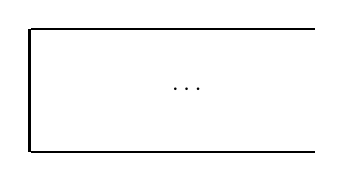
\begin{tikzpicture}[x=0.6cm,y=0.6cm]
  \fill[black] (-0.08,-1.3) rectangle (0,1.3); % 閉端（固定壁）を表す黒い長方形
  \draw[thick] (0,1.3) -- (6,1.3); % 管の上側の壁を表す直線（全体）
  \draw[thick] (0,-1.3) -- (6,-1.3); % 管の下側の壁を表す直線（全体）
  \node[font=\small] at (3.333,0) {$\cdots$}; % 中央部分：多数のループが続くことを省略記号で示す
\end{tikzpicture}}
& & & \\
\cline{2-4}
\end{tabular}

\begin{pointbox}
\textbf{ヒント}：図に引かれた破線(節)・点線(腹)の\textbf{数}に注目する。節と節(または腹と腹)の間隔は $\lambda/2$，節と腹の間隔は $\lambda/4$ である。波長 $\lambda$ が求まれば，$f=\dfrac{V}{\lambda}$ から振動数が求まる。
\end{pointbox}

\end{document}
